\documentclass[a4paper]{article}
\usepackage{polski}
\usepackage[T1]{fontenc}
\usepackage[polish]{babel}
\usepackage[utf8x]{inputenc}
\usepackage{amsmath}
\usepackage{graphicx}
\usepackage[T1]{fontenc}
\usepackage{lmodern}
\usepackage{setspace}
\usepackage[a4paper,left=3cm,right=2cm,top=2.5cm,bottom=2.5cm]{geometry}
\onehalfspacing
\selectlanguage{polish}

\title{Portal społecznościowy}

\author{ Natalia Musiał \and Michał Juszczak \and Mariusz Nyznar\and  Agnieszka Kowal \and Łukasz Kmiecik \and Krzysztof Misiak}


\begin{document}
\maketitle


\section{Grupy}

Projekt zostanie zrealizowany przez 6 osób rozmieszczonych w trzech dwuosobowych grupach .
\subsection{Zespół 1}
\begin{enumerate}
\item Natalia Musiał
\item Agnieszka Kowal
\end{enumerate}
\subsection{Zespół 2}
\begin{enumerate}
\item Łukasz Kmiecik
\item Michał Juszczak
\end{enumerate}
\subsection{Zespół 3}
\begin{enumerate}
\item Mariusz Nyznar
\item Krzysztof Misiak

\end{enumerate}


\section{Koncepcja systemu}

System ma być imitacją popularnego serwisu Twitter umożliwiającego komunikację pomiędzy użytkowanikami za pomocą krótkich wiadomości.
Możliwości systemu:
\begin{itemize}
\item Wysyłanie wiadomości między użytkownikami
\item Oznaczanie \#tagiem wpisów w celu szybszego ich wyszukiwania oraz poszerzania zasięgu wpływu
\item Oznaczanie @tagiem wpisów w celu oznaczenia innych użytkowników
\item Komentowanie postów przez innych użytkowników
\item Możliwość umieszczania adresów URL z filmikami
\item Możliwość umieszczania zdjęć

\end{itemize}



\section{Technologie}
\begin{enumerate}
\item JPA (Hibernate) - ''Java Persistence Api'' to oficjalny standard mapowania obiektowo-relacyjnego (ORM) firmy Sun Microsystems dla języka programowania Java. Hibernate to framework do realizacji warstwy dostępu do danych (ang. persistence layer). Hibernate implementuje JPA.
\item REST - ''Representational State Transfer'' (zmiana stanu poprzez reprezentacje) to styl architektury oprogramowania wywiedziony z doświadczeń przy pisaniu specyfikacji protokołu HTTP dla systemów rozproszonych.
\item JSF + Ajax - ''Java Server Faces'' to framework, bazujący na języku Java, który upraszcza tworzenie interfejsu użytkownika do aplikacji Java EE. ''Asynchronous JavaScript and XML'' to technika tworzenia aplikacji internetowych, w której interakcja użytkownika z serwerem odbywa się bez przeładowywania całego dokumentu, w sposób asynchroniczny.
\item EJB - ''Enterprise JavaBeans'' to komponenty pracujące po stronie serwera aplikacji, zawierające logikę biznesową.
\item CDI - ''Context and Dependency Injection''
\item Bean Validation
\end{enumerate}



\section{Przypadki użycia}
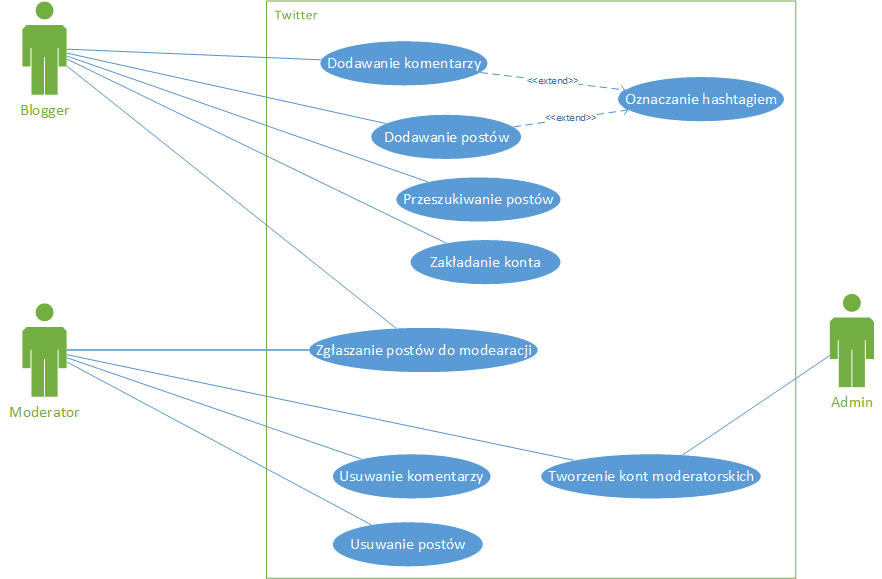
\includegraphics[width=\textwidth]{usecase}
\begin{tabular}{c p{10cm}}
Nazwa& Rejestracja	\\
Numer	& 1\\
Aktorzy & Użytkownik \\
Krótki opis & Użytkownik rejestruje nowe konto \\
Warunki wstępne&  aktywny adres e-mail\\
Warunki końcowe& Użytkownik uzyskuje dostęp do utworzonego konta\\
Główny przepływ zdarzeń&
\begin{enumerate}
\item Użytkownik wybiera opcję ''Register'' na stronie
\item Przeglądarka wyświetla okno rejestracji nowego konta
\item Użytkownik wpisuje nick, hasło oraz e-mail
\item Przegląrka wyświetla komunikat o sukcesie oraz o wysłanym mailu aktywującym na podany adres email
\end{enumerate} \\
Alternatywny przebieg wydarzeń &
3.a Podany nick istnieje w systemie \newline
3.a.1 Przeglądarka wyświetla komunikat z prośbą o wybranie innego nicka\newline
3.b Hasło ma niepoprawny format \newline
3.b.1 Przeglądarka wyświetla komunikat z prośbą o wpisanie hasła w żądanym formacie\newline
3.c Podany e-mail jest już w systemie \newline
3.c.1 Przeglądarka wyświetla komunikat o istnieniu adresu e-mail w systemie \newline
\\
\end{tabular}

\begin{tabular}{c p{10cm}}
Nazwa&	Logowanie\\
Numer	& 2\\
Aktorzy &	Użytkownik\\
Krótki opis &  Użytkownik wpisuje swój nick oraz hasło w celu zalogowania\\
Warunki wstępne&	\\
Warunki końcowe&	Użytkownik uzyskuje dostęp do swojego konta\\
Główny przepływ zdarzeń&
\begin{enumerate}
\item Użytkownik wybiera opcję ''Login'' na stronie
\item Przeglądarka wyświetla okno logowania
\item Użytkownik wpisuje swój nick oraz hasło
\item Przeglądarka wyświetla okno z potwierdzeniem logowania
\item Użytkownik uzyskuje dostęp do konta

\end{enumerate} \\
Alternatywny przebieg wydarzeń &
4.a Użytkownik wpisuje niepoprawne hasło \newline
4.a.1 Przeglądarka wyświetla okno z komunikatem o niepoprawnym haśle \newline
4.a.2 Użytkownik wpisuje ponownie hasło\newline
\\

\end{tabular}


\begin{tabular}{c p{10cm}}
Nazwa&	Wpis\\
Numer	& 3\\
Aktorzy &	Użytkownik\\
Krótki opis &  Użytkownik dodaje wpis na tablicę\\
Warunki wstępne& Użytkownik jest zalogowany\\
Warunki końcowe& Wpis zostaje dodany na tablicę użytkownika, użytkownicy obserwujący mogą go zobaczyć na swoich tablicach\\
Główny przepływ zdarzeń&
\begin{enumerate}
\item Użytkownik wybiera opcję ''\textbf{Napisz nowego posta}''
\item Przeglądarka wyświetla okno nowego wpisu
\item Użytkownik wpisuje tekst w oknie i wybiera opcję wysłania wpisu
\item Przeglądarka zamyka okno wpisu i przeładowuje stronę
\end{enumerate} \\

Alternatywny przebieg wydarzeń &
3.a Użytkownik wpisał zbyt wiele znaków \newline
3.a.1 Przeglądarka blokuje opcję wysłania wpisu i wyświetla komunikat o nadmiarze znaków \newline
3.a.2 Użytkownik skraca wpis \newline
3.a.3 Przeglądarka odblokowuje opcję wysłania \newline
\end{tabular}

\section{Zarys architektury systemu}
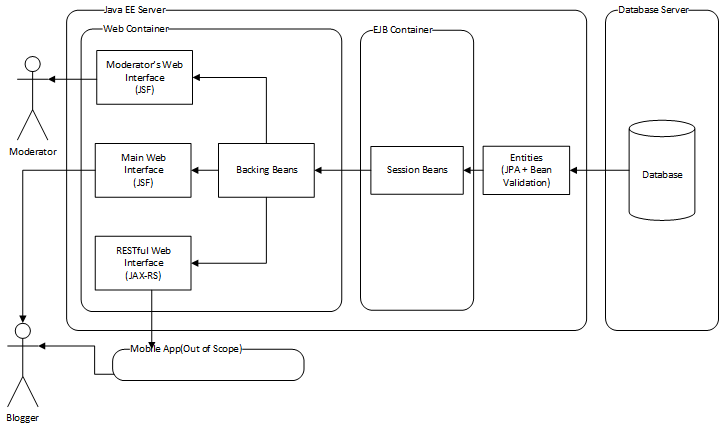
\includegraphics[width=\textwidth]{architecture}
\begin{enumerate}
\item Serwer, do ktorego będą sie łączyć użytkownicy serwisu
\item Baza danych zawierająca wiadomości (posty) użytkownikow
\item Baza danych zawierająca dane użytkowników
\end{enumerate}

\section{Projekt bazy danych}
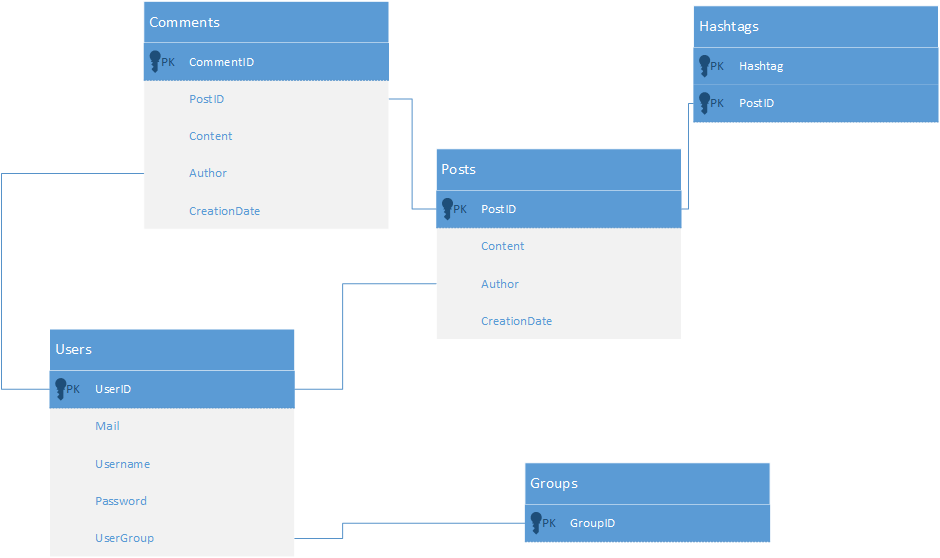
\includegraphics[width=\textwidth]{database}

\section{Słownik pojęć i skrótów}

\begin{tabular}{|p{3cm}| p{7cm}|}
\hline

\hline
\end{tabular}

\end{document}